% coding:utf-8

\documentclass[a4paper,11pt]{article}

\usepackage[utf8]{inputenc} 
\usepackage[T1]{fontenc} 
\usepackage{textcomp} 
%\usepackage{lmodern} 
\usepackage{graphics}
\usepackage{graphicx}
\usepackage[ngermanb]{babel}		
\usepackage{amsmath}
\usepackage{makeidx}
\usepackage{listings}
\usepackage{color}
\usepackage{siunitx}

\definecolor{dkgreen}{rgb}{0, 0.6, 0}
\definecolor{gray}{rgb}{0.5, 0.5, 0.5}
\definecolor{mauve}{rgb}{0.58, 0, 0.82}

% used for code insertions
\lstset{frame=tb,
  language=C,
  aboveskip=3mm,
  belowskip=3mm,
  showstringspaces=false,
  columns=flexible,
  basicstyle={\small\ttfamily},
  numbers=none,
  numberstyle=\tiny\color{gray},
  keywordstyle=\color{blue},
  commentstyle=\color{dkgreen},
  stringstyle=\color{mauve},
  breaklines=true,
  breakatwhitespace=true,
  tabsize=3
}

\title{DSVB - Testataufgabe: Goertzel Algorithmus}
\author{
    Roger Waltenspül \and Daniel Stadelmann
}

\pagestyle{headings}

\begin{document}

\maketitle
\author
\thispagestyle{empty}

\newpage
\pagenumbering{arabic}
\section{Q1 - Q15 Format}
Im Normalfall wird beim umrechnen ins Q15-Format ein Bitshift um 15 Stellen durchgeführt. 
\begin{equation}\label{eq:q15format}
	(a_{Q_{15}} * b_{Q_{15}}) \gg 15 = C_{Q_{15}}
\end{equation}
Dies kann jedoch zu Problemen führen, falls $a_{Q_{15}}$ oder $b_{Q_{15}}$ den Wert $2^{-15}$ annehmen. Wenn einer dieser Werte unser Koeffizient ist und wir garantieren können, dass dieser nie diesen Wert annimmt ist das Shiften um 15 Stellen nach rechts zulässig.
In unserem Code des Goertzel-Algorithmus wird jedoch lediglich um 14 Stellen geshiftet (siehe Code unten). Dies weil die Filterkoeffizienten bei uns im Code als $\frac{a_k}{2}$ definiert wurden. Ein Bitshift um eine Stelle nach rechts entspricht einer Division durch 2 und ist somit nicht mehr notwenig um ins $Q_{15}$-Format umzurechnen.
\begin{lstlisting}
void goertzel_filter_v0 ( short int * delay, short int input, short int coefficient )
{
    long product;

    product = ( (long) delay[1] * coefficient ) >> 14;
    ...
\end{lstlisting}

\section{Q2 - v1 Goertzel Algorithmus}

\section{Q3 - Signal Power Berechnung}

\section{Q4 - Power Calculation Methoden im Vergleich}
\begin{tabular}{lll}
\hline
   & calculation method v0 & calculation method v1 \\
\hline
computational effort    & blabla    & blabla  \\
numerical robustness & blablabla  & blablabla  \\
\hline
\end{tabular}

\section{Todo's}
\subsection{ToDo1}
Die DTMF Frequenzen für die jeweiligen Reihen und Spalten können direkt aus der Definition übernommen werden (siehe Abbildung~\ref{fig:DTMF_freq}).
\begin{figure}[h!]
\centering
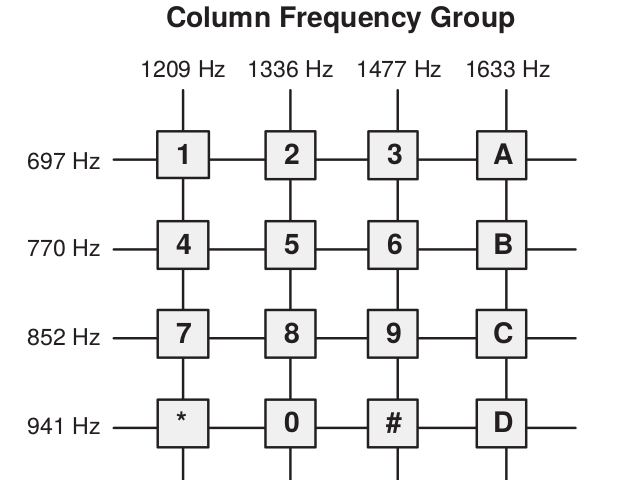
\includegraphics[width=0.5\textwidth]{DTMF_freq}
\caption{DTMF Frequenzen}
\label{fig:DTMF_freq}
\end{figure}
\newline
Der Scalingfaktor lässt sich mit folgender Formel berechnen:
\begin{equation}\label{eq:Scalingfakt}
	Scalingfaktor = \frac{2*(2^{15}-1)}{f_{sample}}*2^{11}
\end{equation}
Bei einer Samplingfrequenz von \SI{8000}{\hertz} ergibt dies einen Wert von 16777. Wichtig ist hier, dass man den Wert als long speichert (16777L). 

\subsection{ToDo2}
Beim Todo 2 mussten die Goertzel-Koeffizienten im $Q_{15}$-Format für die jeweilige Frequenz berechnet werden.
\begin{equation}\label{eq:Goertzel_Koeff}
	\frac{a_k}{2}= \cos(2*\pi*\frac{f_k}{f_s})*2^{15}
\end{equation}
Auch hier beträgt die Abtastfrequenz \SI{8000}{\hertz} und $f_k$ ist die jeweilige Signalfrequenz.

\subsection{ToDo3}
Die Reihenfolge der Zugriffe muss ein wenig umstrukturiert werden. Zuerst wird das Produkt berechnet und der alte Wert delay[2] abgezogen werden. Anschliessend wird der delay Wert um eins geschoben und der neue Wert berechnet und an der Stelle delay[1] abgelegt. 
\begin{lstlisting}
void goertzel_filter_v1 ( short int * delay, short int input, short int coefficient ){
	short int product;

	product = (short int) (( (long) delay[1] * coefficient ) >> 14) - delay[2];

	/* The input is divided by 128 to prevent overload */
	delay[2] = delay[1];
	delay[1] = (short int)( (input >> 7) + product);
}
\end{lstlisting}



\end{document}
